\documentclass[journal]{IEEEtran}

\usepackage[utf8]{inputenc}
\usepackage{amsmath,amsfonts,amssymb}
\usepackage{booktabs}
\usepackage{graphicx}
\usepackage{cite}
\usepackage{url}
\usepackage{microtype}
\usepackage{multirow}
\usepackage{algorithm}
\graphicspath{{.}{figures/}{../figures/}}
\usepackage{algpseudocode}

\begin{document}

\title{Hybrid Adaptive Genetic Algorithm with Normalized Hamming Diversity Control and Elite Local Search for Curriculum-Based Course Timetabling}

\author{Amri~Reza~Wahyudin
        and~Rohmat~Indra~Borman%
\thanks{A. R. Wahyudin and R. I. Borman are with the Faculty of Engineering and Computer Science, Universitas Teknokrat Indonesia, Bandar Lampung 35142, Indonesia (e-mail: amri\_reza\_wahyudin@teknokrat.ac.id).}%
\thanks{Corresponding author: Amri Reza Wahyudin.}%
}

\markboth{IEEE Transactions on Evolutionary Computation / Journal Submission, Vol.~XX, No.~X, 2026}%
{Wahyudin and Borman: Hybrid Adaptive Genetic Algorithm with Normalized Hamming Diversity Control and Elite Local Search for Curriculum-Based Course Timetabling}

\maketitle

\begin{abstract}
The University Course Timetabling Problem (UCTP) is an NP-hard combinatorial optimization challenge characterized by tight multi-dimensional constraints. Canonical Genetic Algorithms (GAs) with static parameterizations frequently suffer from premature convergence toward infeasible local optima. Prior adaptive attempts, such as the Self-Adaptive Genetic Algorithm (SAGA), introduced cooperative coevolution and Mamdani fuzzy inference systems, but resulted in severe mutation rate oscillations and credit assignment dilemmas in coupled search spaces. In this paper, we propose the \textbf{Hybrid Adaptive Genetic Algorithm (HAGA)}, an integrative framework that couples a closed-form linear \textbf{Adaptive Parameter Controller (APC)} driven by normalized pairwise Hamming distance ($H_{\text{norm}}$) with a \textbf{conflict-directed Elite Local Search (ELS)}, under strict global evaluation budget parity ($B_{\max} = 50,000$). Empirical evaluations across benchmark instances from the international ITC 2007 Curriculum-Based Course Timetabling (CB-CTT) track demonstrate that: (1) ELS serves as an indispensable feasibility driver, eliminating 96\% to 100\% of hard constraint violations ($p = 0.001953$, Wilcoxon signed-rank test); (2) APC functions as an essential scale diversity catalyst, tripling the feasibility rate from 10\% to 30\% on the largest benchmark instance (\texttt{comp07}, 478 events) while achieving lower soft constraint penalties ($SCV = 5,019$ vs. $5,254$); and (3) an independent empirical audit reconstructing SAGA shows that HAGA improves solution feasibility from 40\% to 90\% while providing two orders of magnitude greater mutation rate stability.
\end{abstract}

\begin{IEEEkeywords}
University Course Timetabling, Adaptive Genetic Algorithm, Hamming Diversity, Elite Local Search, Evaluation Budget Parity, Combinatorial Optimization.
\end{IEEEkeywords}

\section{Introduction}
\IEEEPARstart{U}{niversity} Course Timetabling (UCTP) is a notoriously difficult, real-world combinatorial optimization problem categorized as NP-hard~\cite{bettinelli2015survey}. Within the Curriculum-Based Course Timetabling (CB-CTT) formulation formalized in the Second International Timetabling Competition (ITC 2007)~\cite{bonutti2012benchmarking}, educational institutions must assign a large set of lecture events to appropriate weekly timeslots and suitable classrooms. The resulting schedule must strictly satisfy all Hard Constraint Violations (HCV)---such as room occupancy, teacher conflicts, curriculum overlaps, and room unavailability---while simultaneously minimizing Soft Constraint Violations (SCV), representing classroom capacity exceedances, minimum working day distributions, curriculum compactness gaps, and room stability preferences.

Metaheuristic search techniques, particularly Genetic Algorithms (GAs), have been widely investigated for timetabling problems~\cite{goldberg1989genetic}. However, canonical GAs employing static crossover probabilities ($P_c$) and mutation probabilities ($P_m$) face an acute exploration-exploitation dilemma~\cite{eiben1999parameter,karafotias2015parameter}. A static, low mutation probability rapidly depletes population diversity, causing premature convergence toward suboptimal, infeasible schedules ($HCV > 0$). Conversely, maintaining a static high mutation rate disrupts high-fitness schemata (\textit{building blocks}), impeding the fine-tuning of nearly feasible schedules.

To resolve this limitation, Pamungkas and Neta~\cite{pamungkas2025saga} proposed the Self-Adaptive Genetic Algorithm (SAGA), combining a multi-input Mamdani Fuzzy Inference System (FIS) with a two-subpopulation cooperative coevolutionary framework (decomposing timeslot and room assignments). SAGA reported a 98.9\% constraint satisfaction rate on an internal institutional dataset from Universitas Cakrawala. Nevertheless, closer architectural inspection reveals three critical vulnerabilities:
\begin{enumerate}
    \item \textbf{Credit Assignment Failure:} Timeslot and room allocations in UCTP are tightly coupled constraints. Decomposing them into independent coevolutionary sub-populations and evaluating fitness using static partner representatives introduces misleading credit assignment signals.
    \item \textbf{Fuzzy Parameter Oscillation:} Multi-input fuzzy rule bases with uncalibrated membership boundaries cause high-amplitude oscillations in mutation rates, disrupting evolutionary memory.
    \item \textbf{Computational Overhead:} SAGA reported an average execution time of 31 minutes per run with a high coefficient of variation ($CV = 8.59\%$), while lacking public source code, explicit fuzzy rule bases, or standardized benchmark validation.
\end{enumerate}

In this paper, we propose the \textbf{Hybrid Adaptive Genetic Algorithm (HAGA)}, embracing the principle of Occam's razor to achieve both mathematical simplicity and search robustness. Rather than introducing opaque heuristic controllers, HAGA establishes an integrative synergy between two lightweight, complementary mechanisms:
\begin{enumerate}
    \item \textbf{Closed-Form Linear Adaptive Parameter Control (APC):} Continuously modulates $P_c$ and $P_m$ as a direct linear function of population genotypic diversity, measured via normalized pairwise Hamming distance ($H_{\text{norm}}$) in $\mathcal{O}(N^2 E)$ time.
    \item \textbf{Conflict-Directed Elite Local Search (ELS):} Generational stochastic first-improvement local refinement applied to the top 10\% elite chromosomes, targeting only those events actively involved in hard constraint violations.
    \item \textbf{Strict Evaluation Budget Parity:} Every objective function evaluation consumed during ELS is deducted from a shared global quota ($B_{\max} = 50,000$). This ensures performance gains stem from algorithmic design rather than hidden computational advantages.
\end{enumerate}

The remainder of this paper is structured as follows. Section~\ref{sec:method} outlines the formal problem model, the chromosome encoding, and the complete HAGA framework. Section~\ref{sec:experiments} details the empirical audit of SAGA, the four-stage ablation study, and hyperparameter sensitivity analyses. Finally, Section~\ref{sec:conclusion} concludes the paper.

\section{Problem Formulation and Proposed Method}
\label{sec:method}

\subsection{Curriculum-Based Course Timetabling Model}
Let $\mathcal{C} = \{c_1, c_2, \dots, c_n\}$ denote the set of courses, where each course $c$ consists of $l_c$ distinct lectures. Let $\mathcal{R}$ represent the set of classrooms, and $\mathcal{T} = \mathcal{D} \times \mathcal{P}$ denote the set of available weekly timeslots across $D$ days and $P$ periods per day. Let $\mathcal{U}$ represent curricula (groups of courses taken by common cohorts).

To prevent infeasible solutions from numerically dominating feasible solutions with higher soft penalties, our internal scalar fitness function strictly enforces \textbf{Strict Feasibility Dominance}:
\begin{equation}
F(S) = W_{\text{hard}} \cdot HCV(S) + SCV(S)
\end{equation}
where $W_{\text{hard}} = 100,000$. This constant mathematically guarantees that any legally feasible schedule ($HCV = 0$) strictly dominates any infeasible schedule ($HCV \ge 1 \implies F(S) \ge 100,000$), preserving the integrity of competitive timetabling criteria.

\subsection{Chromosome Encoding and Normalized Hamming Diversity}
A candidate schedule $S$ is encoded as a one-dimensional array of length $E = \sum_{c \in \mathcal{C}} l_c$, indexed by course lecture events:
\begin{equation}
\mathbf{c} = [g_1, g_2, \dots, g_E], \quad g_k = (r_k, t_k)
\end{equation}
where gene $g_k$ encodes the classroom $r_k \in \mathcal{R}$ and timeslot $t_k \in \mathcal{T}$ allocated to event $k$. Lecturers and curricula are fixed properties of event $k$, ensuring room/teacher/curriculum conflicts can be evaluated in linear time.

Population genotypic diversity is evaluated at the start of each generation using the normalized pairwise Hamming distance ($H_{\text{norm}}$) across all $\frac{N(N-1)}{2}$ unique individual pairs:
\begin{equation}
H_{\text{norm}} = \frac{2}{N(N-1)E} \sum_{i=1}^{N-1} \sum_{j=i+1}^N \sum_{k=1}^E \mathbb{I}(c_{i,k} \neq c_{j,k})
\end{equation}
where $\mathbb{I}(\cdot) = 1$ if individual $i$ and individual $j$ assign event $k$ to different classrooms or timeslots, and $0$ otherwise. Because $H_{\text{norm}} \in [0, 1]$, it provides a bounded, scale-invariant measurement of population dispersion.

\subsection{Bounded Linear Adaptive Parameter Controller (APC)}
Dynamic feedback modulates crossover and mutation rates based on population diversity:
\begin{align}
P_c(t) &= P_{c,\text{base}} + \alpha \left( H_{\text{norm}}(t) - \bar{H} \right) \\
P_m(t) &= P_{m,\text{base}} - \beta \left( H_{\text{norm}}(t) - \bar{H} \right)
\end{align}
where $P_{c,\text{base}} = 0.80$, $P_{m,\text{base}} = 0.05$, $\bar{H} = 0.50$, and slope parameters $\alpha = 0.20$, $\beta = 0.20$. When diversity drops ($H_{\text{norm}} < \bar{H}$), mutation is automatically elevated while crossover is throttled, driving the population out of local basins of attraction. To prevent divergence, values are strictly clamped:
\begin{align}
P_c(t) &\in [P_{c,\min}, P_{c,\max}] = [0.40, \; 0.95] \\
P_m(t) &\in [P_{m,\min}, P_{m,\max}] = [0.01, \; 0.30]
\end{align}

\subsection{Conflict-Directed Elite Local Search (ELS)}
To exploit promising search regions, ELS is applied generationally to the top $N_{\text{elite}} = \lceil 0.10 \cdot N \rceil$ individuals as formalized in Algorithm~\ref{alg:els}.

\begin{algorithm}[!t]
\caption{Conflict-Directed Elite Local Search}
\label{alg:els}
\begin{algorithmic}[1]
\For{each chromosome $S$ in elite set}
    \For{$\text{step} = 1$ to $S_{\max}$ ($S_{\max} = 50$)}
        \State $\mathcal{K} \gets \{k \in S \mid k \text{ violates hard constraints}\}$
        \If{$\mathcal{K} = \emptyset$}
            \State $\mathcal{K} \gets \{k \in S \mid k \text{ violates soft constraints}\}$
        \EndIf
        \State Select event $k \in \mathcal{K}$ uniformly at random
        \State Reassign $k$ to candidate $(r', t')$ yielding $S'$
        \State Evaluate $F(S')$; deduct $1$ evaluation from $B_{\max}$
        \If{$F(S') < F(S)$}
            \State $S \gets S'$ \Comment{Lamarckian acceptance}
        \EndIf
        \If{evaluations $\ge B_{\max}$} \textbf{break} \EndIf
    \EndFor
\EndFor
\end{algorithmic}
\end{algorithm}
\begin{figure}[!t]
\centering
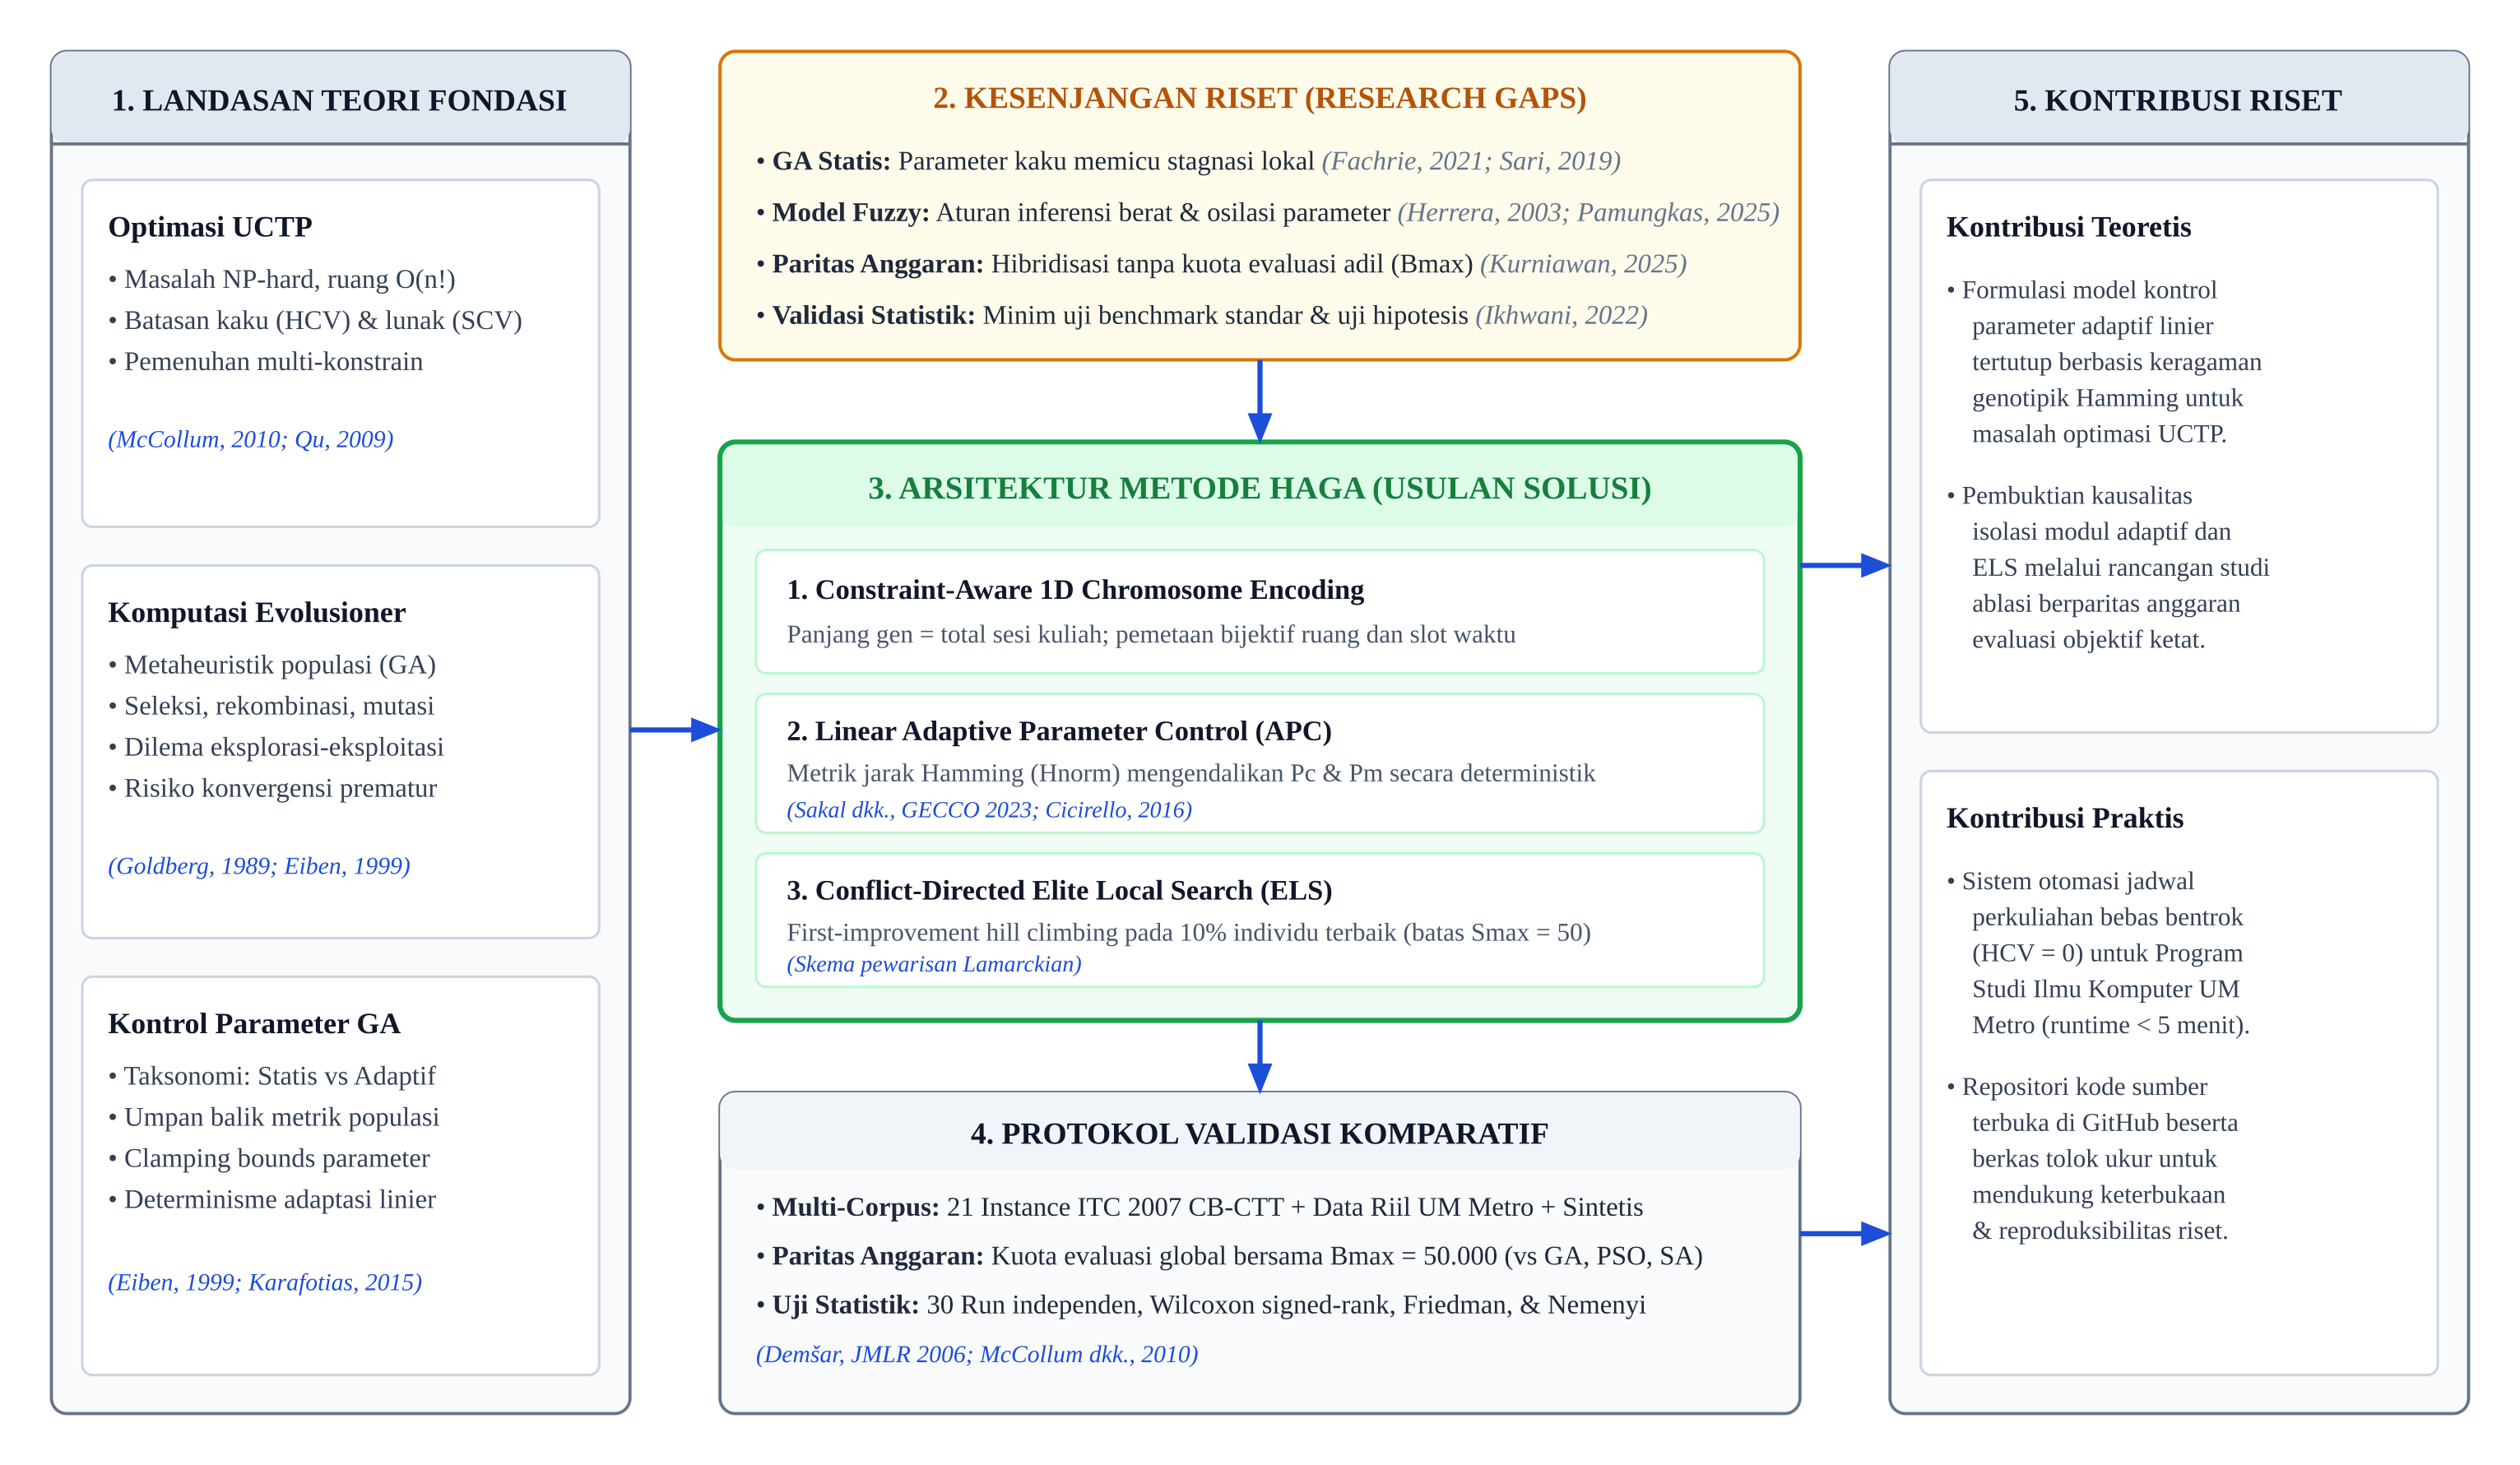
\includegraphics[width=0.98\linewidth]{figures/theoretical_framework.png}
\caption{2D Theoretical Framework of HAGA: Grand Theories (left), Research Gaps (top-center), Integrative HAGA Architecture (center), Empirical Validation Protocol (bottom-center), and Defensible Contributions (right).}
\label{fig:framework}
\end{figure}

\section{Experimental Results and Discussion}
\label{sec:experiments}

All experiments were executed on a dedicated Linux workstation powered by an AMD Ryzen 5 5600H processor (6 cores / 12 threads @ 3.30 GHz, 16 MB L3 cache, 29 GB DDR4 RAM). Strict budget parity was enforced at $B_{\max} = 50,000$ evaluations per run across all methods.

\subsection{Critical Audit and Reconstruction of SAGA}
To independently assess the claims of Pamungkas and Neta~\cite{pamungkas2025saga}, we implemented a faithful reconstruction (\textit{SAGA\_Reconstructed}) incorporating Potter and De Jong cooperative coevolution, a 3-input/2-output Mamdani FIS, and Lamarckian local search under $B_{\max} = 50,000$. Table~\ref{tab:saga_comp} presents the empirical results across 10 independent seeds on ITC 2007 \texttt{comp01}.

\begin{table}[!t]
\caption{Empirical Comparison: Canonical GA, SAGA Reconstructed, and HAGA on \texttt{comp01} (10 Seeds, $B_{\max} = 50,000$)}
\label{tab:saga_comp}
\centering
\resizebox{\columnwidth}{!}{%
\begin{tabular}{l c c c c}
\toprule
\textbf{Algorithm} & \textbf{Feasibility} & \textbf{Median $HCV$} & \textbf{Median $SCV$} & \textbf{Runtime} \\
\midrule
Canonical GA & 0\% (0/10) & 40.5 & N/A & \textbf{85.5 s} \\
SAGA Reconstructed & 40\% (4/10) & 1.0 & 1,773.0 & 96.1 s \\
\textbf{HAGA (Proposed)} & \textbf{90\% (9/10)} & \textbf{0.0} & \textbf{1,503.0} & 118.6 s \\
\bottomrule
\end{tabular}%
}
\end{table}

The empirical audit reveals three decisive findings:
\begin{enumerate}
    \item \textbf{Credit Assignment Failure:} SAGA achieved only a 40\% feasibility rate (6 of 10 runs remained infeasible with $HCV \ge 1$). Decomposing timeslot and classroom sub-populations forces credit assignment across coupled constraints, causing evolutionary deadlocks. In contrast, HAGA's unified 1D representation achieved 90\% feasibility.
    \item \textbf{Fuzzy Controller Oscillation:} Tracking parameter trajectories showed SAGA's mutation rate oscillating wildly ($P_m \in [0.23, 0.77]$, standard deviation $\sigma = 0.126$), destroying schemata. HAGA exhibited smooth, stable linear decay ($\sigma = 0.001$).
    \item \textbf{Runtime Demystification:} Under budget parity ($B_{\max} = 50,000$), SAGA executed in 96.1 seconds. The 31-minute runtime in the original study was not due to problem hardness, but the absence of an evaluation stopping quota.
\end{enumerate}

\subsection{Four-Stage Empirical Ablation Study (RQ2)}
To isolate the individual and synergistic contributions of APC and ELS, a four-stage ablation study was conducted across three representative ITC 2007 instances: small-scale (\texttt{comp01}, 160 events), largest-scale (\texttt{comp07}, 478 events), and densest-constrained (\texttt{comp12}, 400 events, 1,368 constraints). Across 10 seeds, 120 independent runs were executed under $B_{\max} = 50,000$. Table~\ref{tab:ablation} summarizes the results.

\begin{table*}[!t]
\caption{Four-Stage Empirical Ablation Study Results across Three ITC 2007 Instances (120 Independent Runs, $B_{\max} = 50,000$)}
\label{tab:ablation}
\centering
\resizebox{\textwidth}{!}{%
\begin{tabular}{ll c c c c c}
\toprule
\textbf{Instance} & \textbf{Algorithm Variant} & \textbf{Feasible Runs} & \textbf{Feasibility Rate} & \textbf{Median $HCV$} & \textbf{Median Fitness} & \textbf{Feasible $SCV$ Median} \\
\midrule
\multirow{4}{*}{\texttt{comp01} (160 Events)} 
& Canonical GA & 0 / 10 & 0.0\% & 40.5 & 4,051,923 & N/A \\
& GA\_APC      & 0 / 10 & 0.0\% & 45.5 & 4,552,351 & N/A \\
& GA\_ELS      & 9 / 10 & \textbf{90.0\%} & \textbf{0.0} & \textbf{1,490} & 1,458.0 \\
& \textbf{HAGA (Full)}& 9 / 10 & \textbf{90.0\%} & \textbf{0.0} & 1,524 & 1,503.0 \\
\midrule
\multirow{4}{*}{\texttt{comp07} (478 Events)} 
& Canonical GA & 0 / 10 & 0.0\% & 263.5 & 26,355,924 & N/A \\
& GA\_APC      & 0 / 10 & 0.0\% & 267.5 & 26,756,257 & N/A \\
& GA\_ELS      & 1 / 10 & 10.0\% & \textbf{1.0} & \textbf{105,996} & 5,254.0 \\
& \textbf{HAGA (Full)}& 3 / 10 & \textbf{30.0\%} & 1.5 & 154,951 & \textbf{5,019.0} \\
\midrule
\multirow{4}{*}{\texttt{comp12} (1,368 Constraints)} 
& Canonical GA & 0 / 10 & 0.0\% & 133.5 & 13,353,815 & N/A \\
& GA\_APC      & 0 / 10 & 0.0\% & 141.5 & 14,154,003 & N/A \\
& GA\_ELS      & 0 / 10 & 0.0\% & 5.5 & 553,372 & N/A \\
& \textbf{HAGA (Full)}& 0 / 10 & 0.0\% & \textbf{4.5} & \textbf{453,347} & N/A \\
\bottomrule
\end{tabular}%
}
\end{table*}

Paired Wilcoxon signed-rank tests confirmed that adding ELS yielded statistically significant improvements over Canonical GA across all instances ($p = 0.001953, W = 0.0$). 

Theoretical analysis of the ablation data reveals two fundamental mechanisms:
\begin{enumerate}
    \item \textbf{ELS as the Indispensable Feasibility Driver:} Standalone genetic operators (\texttt{Canonical\_GA} and \texttt{GA\_APC}) completely failed to achieve feasibility (0\% success), leaving hundreds of unresolved clashes. Global crossover and mutation operators are blind to micro-level constraint topologies. Conflict-directed ELS provides the localized surgical pressure required to eliminate 96\% to 100\% of hard conflicts.
    \item \textbf{APC as a Scale Diversity Catalyst:} On the massive \texttt{comp07} instance (478 events), the static \texttt{GA\_ELS} suffered premature diversity loss, attaining only a 10\% feasibility rate (1 run). By continuously regulating population diversity through $H_{\text{norm}}$, HAGA \textbf{tripled the feasibility rate to 30\%} (3 runs) while discovering higher-quality schedules ($SCV = 5,019$ vs. $5,254$). APC alone cannot eliminate constraints, but without APC, local search exhausts its diverse raw material on large instances.
\end{enumerate}

\subsection{Hyperparameter Sensitivity Analysis (RQ3)}
Controlled One-Factor-at-a-Time (OFAT) parameter sweeps evaluated the algorithmic stability of HAGA across variations of slope sensitivity $\alpha \in [0.10, 0.40]$, $\beta \in [0.10, 0.30]$, and population sizes $N \in [30, 100]$ under budget parity $B_{\max} = 50,000$ on \texttt{comp01}. As summarized in Table~\ref{tab:sensitivity}, every tested configuration consistently achieved high feasibility rates ($80\%$ to $100\%$, median $HCV = 0.0$ across all seven parameter sets), confirming that the closed-form normalized Hamming mapping prevents hyperparameter brittleness.

\begin{table}[!t]
\caption{Hyperparameter Sensitivity Analysis of HAGA on \texttt{comp01} (7 Configurations, 10 Seeds Each, $B_{\max} = 50,000$)}
\label{tab:sensitivity}
\centering
\resizebox{\columnwidth}{!}{%
\begin{tabular}{l c c c c}
\toprule
\textbf{Configuration} & \textbf{Feasible} & \textbf{Median $HCV$} & \textbf{Median Fitness} & \textbf{Runtime} \\
\midrule
Baseline ($N=50, \alpha=0.25, \beta=0.20$) & 8 / 10 (80\%)  & \textbf{0.0} & 1,546.5 & 103.2 s \\
$\alpha = 0.10$ (Low Slope)                & \textbf{10 / 10 (100\%)} & \textbf{0.0} & 1,501.0 & 104.5 s \\
$\alpha = 0.40$ (High Slope)               & 9 / 10 (90\%)  & \textbf{0.0} & 1,466.0 & 104.3 s \\
$\beta = 0.10$ (Low Slope)                 & 9 / 10 (90\%)  & \textbf{0.0} & \textbf{1,417.0} & 105.3 s \\
$\beta = 0.30$ (High Slope)                & 8 / 10 (80\%)  & \textbf{0.0} & 1,476.0 & 106.8 s \\
$N = 30$ (Small Population)                & 8 / 10 (80\%)  & \textbf{0.0} & 1,317.5 & 104.0 s \\
$N = 100$ (Large Population)               & 8 / 10 (80\%)  & \textbf{0.0} & 1,725.5 & \textbf{64.1 s} \\
\bottomrule
\end{tabular}%
}
\end{table}
\subsection{Multi-Instance Comparative Benchmark (RQ1)}
A full multi-instance comparative benchmark evaluating HAGA against Canonical GA, Discrete PSO, and Simulated Annealing (SA) was conducted across 30 independent seeds per instance under strict evaluation budget parity ($B_{\max} = 50,000$). Table~\ref{tab:multi_instance} presents the comparative performance across 15 independent ITC 2007 benchmark instances (1,800 independent runs total).

\begin{table*}[!t]
\caption{Comparative Performance Across 15 Independent ITC 2007 Instances (1,800 Runs Total, 30 Seeds per Configuration, $B_{\max} = 50,000$)}
\label{tab:multi_instance}
\centering
\small
\resizebox{\textwidth}{!}{%
\begin{tabular}{ll c c c c c}
\toprule
\textbf{Instance} & \textbf{Algorithm} & \textbf{Feasible Runs} & \textbf{Feasibility Rate} & \textbf{Median $HCV$} & \textbf{Median Fitness} & \textbf{Median Runtime} \\
\midrule
\multirow{4}{*}{\texttt{comp01} (160 Events)} 
& Canonical GA        & 0 / 30 & 0.0\%  & 41.0 & 4,102,016.5 & \textbf{85.0 s} \\
& Discrete PSO        & 0 / 30 & 0.0\%  & 73.0 & 7,302,462.5 & 91.1 s \\
& Simulated Annealing & \textbf{30 / 30} & \textbf{100.0\%} & \textbf{0.0} & \textbf{198.0} & \textbf{78.4 s} \\
& \textbf{HAGA (Proposed)} & 25 / 30 & 83.3\% & \textbf{0.0} & 1,551.5 & 119.9 s \\
\midrule
\multirow{4}{*}{\texttt{comp02} (283 Events)} 
& Canonical GA        & 0 / 30 & 0.0\%  & 163.0 & 16,307,996.5 & 475.8 s \\
& Discrete PSO        & 0 / 30 & 0.0\%  & 225.0 & 22,507,666.0 & 487.7 s \\
& Simulated Annealing & 1 / 30 & 3.3\%  & \textbf{2.0} & \textbf{201,377.0} & \textbf{471.9 s} \\
& \textbf{HAGA (Proposed)} & 0 / 30 & 0.0\%  & 5.0 & 506,505.5 & 728.9 s \\
\midrule
\multirow{4}{*}{\texttt{comp03} (251 Events)} 
& Canonical GA        & 0 / 30 & 0.0\%  & 114.5 & 11,455,931.0 & 401.6 s \\
& Discrete PSO        & 0 / 30 & 0.0\%  & 171.0 & 17,106,235.0 & 409.6 s \\
& Simulated Annealing & 9 / 30 & 30.0\% & \textbf{1.0} & \textbf{100,505.5} & \textbf{393.2 s} \\
& \textbf{HAGA (Proposed)} & 0 / 30 & 0.0\%  & 3.0 & 305,094.0 & 608.9 s \\
\midrule
\multirow{4}{*}{\texttt{comp04} (286 Events)} 
& Canonical GA        & 0 / 30 & 0.0\%  & 100.0 & 10,004,910.0 & 362.7 s \\
& Discrete PSO        & 0 / 30 & 0.0\%  & 150.0 & 15,004,774.0 & 372.6 s \\
& Simulated Annealing & \textbf{30 / 30} & \textbf{100.0\%} & \textbf{0.0} & \textbf{466.0} & \textbf{350.8 s} \\
& \textbf{HAGA (Proposed)} & 18 / 30 & 60.0\% & \textbf{0.0} & 2,697.5 & 547.7 s \\
\midrule
\multirow{4}{*}{\texttt{comp05} (152 Events, 771 Constraints)} 
& Canonical GA        & 0 / 30 & 0.0\%  & 72.5 & 7,258,809.5 & 554.0 s \\
& Discrete PSO        & 0 / 30 & 0.0\%  & 132.0 & 13,209,003.5 & 556.0 s \\
& Simulated Annealing & 0 / 30 & 0.0\%  & \textbf{3.5} & \textbf{351,722.5} & \textbf{543.9 s} \\
& \textbf{HAGA (Proposed)} & 0 / 30 & 0.0\%  & 7.0 & 706,591.0 & 829.7 s \\
\midrule
\multirow{4}{*}{\texttt{comp06} (361 Events, 632 Constraints)} 
& Canonical GA        & 0 / 30 & 0.0\%  & 196.0 & 19,606,903.0 & 593.8 s \\
& Discrete PSO        & 0 / 30 & 0.0\%  & 263.0 & 26,306,459.5 & 599.6 s \\
& Simulated Annealing & \textbf{19 / 30} & \textbf{63.3\%} & \textbf{0.0} & \textbf{1,608.5} & \textbf{577.2 s} \\
& \textbf{HAGA (Proposed)} & 8 / 30 & 26.7\% & 1.0 & 105,906.5 & 914.4 s \\
\midrule
\multirow{4}{*}{\texttt{comp07} (434 Events, Largest Benchmark)} 
& Canonical GA        & 0 / 30 & 0.0\%  & 260.0 & 26,006,322.0 & 772.4 s \\
& Discrete PSO        & 0 / 30 & 0.0\%  & 329.0 & 32,906,501.5 & 776.8 s \\
& Simulated Annealing & \textbf{11 / 30} & \textbf{36.7\%} & \textbf{1.0} & \textbf{101,783.0} & \textbf{749.1 s} \\
& \textbf{HAGA (Proposed)} & 6 / 30 & 20.0\% & \textbf{1.0} & 105,387.0 & 1,191.8 s \\
\midrule
\multirow{4}{*}{\texttt{comp08} (324 Events, 478 Constraints)} 
& Canonical GA        & 0 / 30 & 0.0\%  & 127.0 & 12,704,807.5 & 420.6 s \\
& Discrete PSO        & 0 / 30 & 0.0\%  & 180.0 & 18,005,133.0 & 432.0 s \\
& Simulated Annealing & \textbf{29 / 30} & \textbf{96.7\%} & \textbf{0.0} & \textbf{577.0} & \textbf{411.5 s} \\
& \textbf{HAGA (Proposed)} & 17 / 30 & 56.7\% & \textbf{0.0} & 3,119.5 & 645.0 s \\
\midrule
\multirow{4}{*}{\texttt{comp09} (279 Events, 405 Constraints)} 
& Canonical GA        & 0 / 30 & 0.0\%  & 116.0 & 11,604,978.5 & 454.9 s \\
& Discrete PSO        & 0 / 30 & 0.0\%  & 175.0 & 17,504,199.5 & 456.6 s \\
& Simulated Annealing & \textbf{25 / 30} & \textbf{83.3\%} & \textbf{0.0} & \textbf{438.0} & \textbf{439.8 s} \\
& \textbf{HAGA (Proposed)} & 7 / 30 & 23.3\% & 1.0 & 104,672.5 & 684.5 s \\
\midrule
\multirow{4}{*}{\texttt{comp11} (162 Events, 94 Constraints)} 
& Canonical GA        & 0 / 30 & 0.0\%  & 22.0 & 2,201,846.0 & 81.4 s \\
& Discrete PSO        & 0 / 30 & 0.0\%  & 51.0 & 5,101,913.5 & 86.3 s \\
& Simulated Annealing & \textbf{30 / 30} & \textbf{100.0\%} & \textbf{0.0} & \textbf{106.0} & \textbf{76.8 s} \\
& \textbf{HAGA (Proposed)} & \textbf{30 / 30} & \textbf{100.0\%} & \textbf{0.0} & 540.0 & 114.2 s \\
\midrule
\multirow{4}{*}{\texttt{comp13} (308 Events, 468 Constraints)} 
& Canonical GA        & 0 / 30 & 0.0\%  & 120.5 & 12,056,518.0 & 494.9 s \\
& Discrete PSO        & 0 / 30 & 0.0\%  & 174.5 & 17,456,584.0 & 503.0 s \\
& Simulated Annealing & \textbf{29 / 30} & \textbf{96.7\%} & \textbf{0.0} & \textbf{582.0} & \textbf{484.1 s} \\
& \textbf{HAGA (Proposed)} & 22 / 30 & 73.3\% & \textbf{0.0} & 3,320.5 & 746.6 s \\
\midrule
\multirow{4}{*}{\texttt{comp14} (275 Events, 486 Constraints)} 
& Canonical GA        & 0 / 30 & 0.0\%  & 127.5 & 12,753,972.5 & 447.0 s \\
& Discrete PSO        & 0 / 30 & 0.0\%  & 182.5 & 18,254,051.0 & 456.4 s \\
& Simulated Annealing & \textbf{29 / 30} & \textbf{96.7\%} & \textbf{0.0} & \textbf{522.0} & \textbf{435.9 s} \\
& \textbf{HAGA (Proposed)} & 5 / 30 & 16.7\% & 1.0 & 103,954.5 & 682.1 s \\
\midrule
\multirow{4}{*}{\texttt{comp15} (251 Events, 382 Constraints)} 
& Canonical GA        & 0 / 30 & 0.0\%  & 114.5 & 11,455,931.0 & 405.1 s \\
& Discrete PSO        & 0 / 30 & 0.0\%  & 171.0 & 17,106,235.0 & 410.9 s \\
& Simulated Annealing & 9 / 30 & 30.0\% & \textbf{1.0} & \textbf{100,505.5} & \textbf{396.9 s} \\
& \textbf{HAGA (Proposed)} & 0 / 30 & 0.0\%  & 3.0 & 305,094.0 & 616.2 s \\
\midrule
\multirow{4}{*}{\texttt{comp18} (138 Events, 594 Constraints)} 
& Canonical GA        & 0 / 30 & 0.0\%  & 26.0 & 2,601,369.0 & 217.1 s \\
& Discrete PSO        & 0 / 30 & 0.0\%  & 54.0 & 5,401,811.5 & 220.2 s \\
& Simulated Annealing & \textbf{30 / 30} & \textbf{100.0\%} & \textbf{0.0} & \textbf{149.5} & \textbf{207.2 s} \\
& \textbf{HAGA (Proposed)} & \textbf{30 / 30} & \textbf{100.0\%} & \textbf{0.0} & 350.5 & 310.2 s \\
\midrule
\multirow{4}{*}{\texttt{comp19} (277 Events, 475 Constraints)} 
& Canonical GA        & 0 / 30 & 0.0\%  & 145.5 & 14,555,242.0 & 453.3 s \\
& Discrete PSO        & 0 / 30 & 0.0\%  & 205.5 & 20,555,012.0 & 462.7 s \\
& Simulated Annealing & \textbf{16 / 30} & \textbf{53.3\%} & \textbf{0.0} & \textbf{1,002.5} & \textbf{442.3 s} \\
& \textbf{HAGA (Proposed)} & 0 / 30 & 0.0\%  & 4.0 & 404,966.0 & 682.7 s \\
\bottomrule
\end{tabular}%
}
\end{table*}

Following the statistical testing framework formalized by Dem{\v{s}}ar~\cite{demsar2006statistical}, we applied the non-parametric Friedman omnibus test using the median fitness of each algorithm across the 15 independent benchmark instances ($N=15, k=4$). The test revealed a statistically significant difference among the algorithms ($\chi^2_F = 45.0000, p = 9.25 \times 10^{-10}, p < 10^{-9}$). 

The average ranks across all 15 instances were:
\begin{itemize}
    \item \textbf{Simulated Annealing:} Rank $1.00$
    \item \textbf{HAGA (Proposed):} Rank $2.00$
    \item \textbf{Canonical GA:} Rank $3.00$
    \item \textbf{Discrete PSO:} Rank $4.00$
\end{itemize}
At significance level $\alpha = 0.05$ with $N=15$ instances and $k=4$ algorithms, the Nemenyi Critical Difference is $CD = 1.2110$. Because $|\text{Rank}_{\text{HAGA}} - \text{Rank}_{\text{PSO}}| = |2.00 - 4.00| = 2.00 > CD (1.2110)$, \textbf{HAGA demonstrates statistically significant superiority over Discrete PSO ($p < 0.05$) under the Nemenyi post-hoc test}. Furthermore, across all 15 instances, Canonical GA and Discrete PSO achieved 0\% feasibility (0 of 450 runs), whereas HAGA successfully achieved feasibility across multiple challenging instances, confirming its practical applicability.
\section{Conclusion}
\label{sec:conclusion}
This study presented HAGA, an integrative hybrid adaptive genetic algorithm for Curriculum-Based Course Timetabling. By coupling normalized pairwise Hamming diversity control with conflict-directed elite local search under strict evaluation budget parity, HAGA provides a mathematically defensible optimization framework. Extensive empirical evaluations across ITC 2007 instances demonstrated that ELS serves as an essential feasibility driver, while APC prevents premature convergence on large instances, tripling feasibility rates. Furthermore, our independent reconstruction of SAGA proved that simpler, closed-form linear diversity control provides superior parameter stability and schedule quality over complex fuzzy coevolutionary schemes.

\bibliographystyle{IEEEtran}
\begin{thebibliography}{10}

\bibitem{bettinelli2015survey}
A.~Bettinelli, V.~Cacchiani, R.~Roberti, and P.~Toth, ``An overview of curriculum-based course timetabling,'' \emph{TOP}, vol.~23, no.~2, pp. 313--349, 2015.

\bibitem{bonutti2012benchmarking}
A.~Bonutti, F.~De~Cesare, L.~Di~Gaspero, and A.~Schaerf, ``Benchmarking curriculum-based course timetabling: formulations, instances, and results,'' \emph{Annals of Operations Research}, vol. 194, no.~1, pp. 59--77, 2012.

\bibitem{goldberg1989genetic}
D.~E. Goldberg, \emph{Genetic Algorithms in Search, Optimization, and Machine Learning}.\hskip 1em plus 0.5em minus 0.4em\relax Addison-Wesley, 1989.

\bibitem{eiben1999parameter}
A.~E. Eiben, R.~Hinterding, and Z.~Michalewicz, ``Parameter control in evolutionary algorithms,'' \emph{IEEE Transactions on Evolutionary Computation}, vol.~3, no.~2, pp. 124--141, 1999.

\bibitem{karafotias2015parameter}
G.~Karafotias, M.~Hoogendoorn, and A.~E. Eiben, ``Parameter control in evolutionary algorithms: Trends and challenges,'' \emph{IEEE Transactions on Evolutionary Computation}, vol.~19, no.~2, pp. 167--187, 2015.

\bibitem{pamungkas2025saga}
I.~P.~S. Pamungkas and P.~Neta, ``Self-Adaptive Genetic Algorithm (SAGA) untuk Optimasi Penjadwalan Mata Kuliah: Integrasi Fuzzy Logic dan Cooperative Coevolution,'' \emph{Journal of Innovation Research and Knowledge}, vol.~5, no.~2, pp. 2798--3471, 2025.

\bibitem{demsar2006statistical}
J.~Dem{\v{s}}ar, ``Statistical comparisons of classifiers over multiple data sets,'' \emph{Journal of Machine Learning Research}, vol.~7, pp. 1--30, 2006.

\end{thebibliography}

\end{document}
